\documentclass{article}
\usepackage{tikz}
\newcommand{\startv}{.8}

\begin{document}

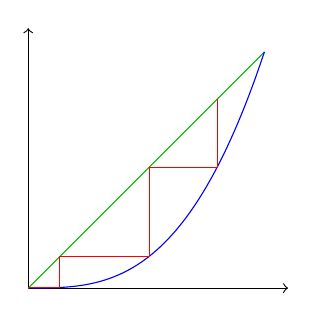
\begin{tikzpicture}[scale=3,declare function={f(\x)=\x*\x*\x;}]
\draw[<->](0,1.1)|-(1.1,0);
\draw[green!70!black] (0,0)--(1,1);
\draw[blue, domain=0:1, smooth] plot (\x,{f(\x)});
\foreach \t[evaluate=\t as \newv using f(\startv)] in {1,...,4}{
    \draw[red] (\startv,\startv)|-(\newv,\newv);
    \xdef\startv{\newv}}
\end{tikzpicture}

\end{document}